
\documentclass[]{report}

\voffset=-1.5cm
\oddsidemargin=0.0cm
\textwidth = 480pt

\usepackage{framed}
\usepackage{subfiles}
\usepackage{graphics}
\usepackage{newlfont}
\usepackage{eurosym}
\usepackage{amsmath,amsthm,amsfonts}
\usepackage{amsmath}
\usepackage{enumerate}
\usepackage{color}
\usepackage{multicol}
\usepackage{amssymb}
\usepackage{multicol}
\usepackage[dvipsnames]{xcolor}
\usepackage{graphicx}
\begin{document}

\section*{Decision Theory }
\begin{itemize}
    \item A decision process is a process requiring either a single or sequential set of decisions for its completion. Each allowable decision has a gain or loss associated with it which is codetermined by external circumstances surrounding the process. 
    \item The set of possible circumstances, known as the states of nature, and a probability distribution governing the occurrence of each state are presumed known.
    \item Both the set of allowable decisions and the set of states of nature will be assumed finite an assumption not made in the more elaborate theory). 
    \item We denote the allowable decisions by $D_1, D_2, \ldots ,D_m$; the states of nature by $S_1, S_2, \ldots ,S_m$ and the return associated with decision and state $S_j$ by $g_{ij}$ (where $ i \in 1,2,m$ and $j \in 1,2,\ldots,n$). 
    \item A process requiring the implementation of just one decision is defined completely by the figure below (Table 18-1). This payoff table is known as a gain matrix whenever the entries $g_{ij}$ are in terms of gains to the decision maker. Losses are then represented as negative gains. 
\end{itemize} 
	\begin{figure}[h!]
\centering
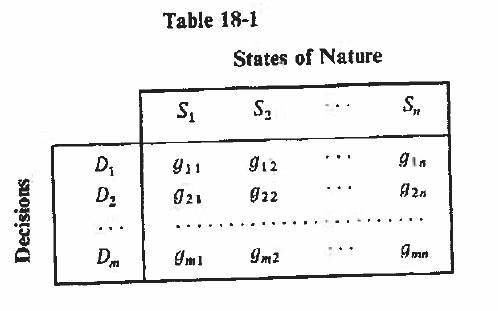
\includegraphics[width=0.4\linewidth]{images/A18-325-A}
%\caption{}
%\label{fig:349-a}
\end{figure}

\section*{Binary Classification}
\subsection*{What Is Classification}
Classification is the problem of identifying to which of a set of categories
(sub-populations) a new observation belongs, on the basis of a training set
of data containing observations (or instances) whose category membership is
known. Binary Classification is the task of classifying the members of a given set of objects into two groups on the basis
if them having a particular set of characteristics.

% Logisticn Rege Discriminant analysis is an example of a classification method.
\begin{itemize}
\item  To train (create) a classifier, the fitting function estimates the parameters
of a Gaussian distribution for each class.
\item  To predict the classes of new data, the trained classifier finds the class
with the smallest misclassification cost.
\end{itemize}
\subsection*{Types I and II Error}
A type I error is the incorrect rejection of a true null hypothesis. A type
II error is the failure to reject a false null hypothesis. A type I error is a
false positive. Usually a type I error leads one to conclude that a thing or
relationship exists when really it doesn’t. A type II error is a false negative.
\begin{figure}[h!]
\centering
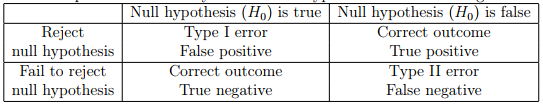
\includegraphics[width=0.7\linewidth]{images/Table}
% \caption{}
% \label{fig:table}
\end{figure}






%------------------------------------------------------%
% http://www.psychwiki.com/wiki/Analyzing_Data
% http://www.upa.pdx.edu/IOA/newsom/semclass/ho_missing.pdf
% http://www.uvm.edu/~dhowell/StatPages/More_Stuff/Missing_Data/Missing.html
% http://www.uvm.edu/~dhowell/StatPages/More_Stuff/Missing_Data/Missing.html
% http://www.stat.columbia.edu/~gelman/arm/missing.pdf
% https://onlinecourses.science.psu.edu/stat505/node/78
% http://rer.sagepub.com/content/45/4/543.full.pdf
% http://www.kdnuggets.com/faq/precision-recall.html
\section{Classification}
\subsection{What Is Classification}
classification is the problem of identifying to which of a set of categories (sub-populations) a new observation belongs, on the basis of a training set of data containing observations (or instances) whose category membership is known.
Discriminant analysis is an example of a \textbf{classification} method.

% It assumes that different classes generate data based on different Gaussian distributions.

\begin{itemize}
\item To train (create) a classifier, the fitting function estimates the parameters of a Gaussian distribution for each class.
\item To predict the classes of new data, the trained classifier finds the class with the smallest misclassification cost.
\end{itemize}
%-----------------------------------------------------------------------------------%
%\subsection{Recall and Precision}
%
%In a classification task, the precision for a class is the number of true positives (i.e. the number of items correctly labeled as belonging to the positive class) divided by the total number of elements labeled as belonging to the positive class (i.e. the sum of true positives and false positives, which are items incorrectly labeled as belonging to the class). Recall in this context is defined as the number of true positives divided by the total number of elements that actually belong to the positive class (i.e. the sum of true positives and false negatives, which are items which were not labeled as belonging to the positive class but should have been).



%-----------------------------------------------------------------------%
\subsection{Types I and II Error}
A type I error is the incorrect rejection of a true null hypothesis.
A type II error is the failure to reject a false null hypothesis.
A type I error is a false positive. Usually a type I error leads one to conclude that a thing
or relationship exists when really it doesn't.
A type II error is a false negative.
\begin{tabular}{|c|c|c|}
  \hline
  % after \\: \hline or \cline{col1-col2} \cline{col3-col4} ...

& Null hypothesis ($H_0$) is true	& Null hypothesis ($H_0$) is false\\ \hline
Reject  & Type I error          & Correct outcome \\
null hypothesis 			& False positive	& True positive\\ \hline
Fail to reject 	&Correct outcome&Type II error\\
null hypothesis & True negative	& False negative\\
  \hline
\end{tabular}
%-----------------------------------------------------------------------%
\subsection{False Positive and False Negative error}

A false positive error, commonly called a ``false alarm" is a result that indicates a
given condition has been fulfilled, when it actually has not been fulfilled.
A false positive error is a \textbf{Type I error} where the test is checking a single condition,
and results in an affirmative or negative decision usually designated as "true or false".

A false negative error is where a test result indicates that a condition failed, while it actually was successful.
A false negative error is a \textbf{Type II error} occurring in test steps where a single
condition is checked for and the result can either be positive or negative.


\subsection{Confusion Matrix}

A \textbf{confusion matrix}, is a table with two rows and two columns that reports the number of false positives, false negatives, true positives, and true negatives.

This allows more detailed analysis than mere proportion of correct guesses (accuracy). Accuracy is not a reliable metric for the real performance of a classifier, because it will yield misleading results if the data set is unbalanced (that is, when the number of samples in different classes vary greatly).

For example, if there were 95 cats and only 5 dogs in the data set, the classifier could easily be biased into classifying all the samples as cats. The overall accuracy would be 95\%, but  in practice the classifier would have a 100\% recognition rate for the cat class but a 0\% recognition rate for the dog class.

%-------------------------------------------------------------------------------------%

\subsection{Sensitivity and Specificity}

Sensitivity and specificity are measures of the performance of a binary classification test.

\begin{itemize}
\item Sensitivity (also called the true positive rate, or the \textbf{recall} rate) measures the proportion of actual positives which are correctly identified as such (e.g. the percentage of sick people who are correctly identified as having the condition).
    \[ \mbox{sensitivity (Recall)} = \frac{ \mbox{number of true positives} } {\mbox{number of true positives} + \mbox{number of false negatives}} \]

\item Specificity measures the proportion of negatives which are correctly identified as such (e.g. the percentage of healthy people who are correctly identified as not having the condition, sometimes called the true negative rate).
    \[ \mbox{ Specificity} = \frac{ \mbox{number of true negatives} } {\mbox{number of false positives} + \mbox{number of true negatives}} \]

\end{itemize}

(Remark: We will use the terms \textbf{Sensitivity} and \textbf{Recall} interchangeably. Sensitivity is more commonly used in a medical context, while recall is more commonly used in data science.)

\subsection{Receiver Operating Characteristic (ROC) curve }


In a Receiver Operating Characteristic (ROC) curve the true positive rate (Sensitivity) is plotted in function of the false positive rate (100-Specificity) for different cut-off points. Each point on the ROC curve represents a sensitivity/specificity pair corresponding to a particular decision threshold. A test with perfect discrimination (no overlap in the two distributions) has a ROC curve that passes through the upper left corner (100\% sensitivity, 100\% specificity). Therefore the closer the ROC curve is to the upper left corner, the higher the overall accuracy of the test (Zweig and Campbell, 1993).

\begin{figure}
  % Requires \usepackage{graphicx}
  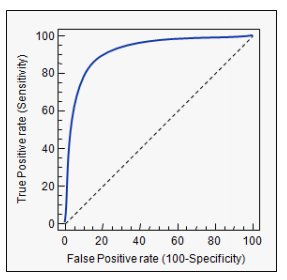
\includegraphics[scale=0.7]{images/ROCcurve.PNG}\\
  \caption{Receiver Operating Characteristic (ROC) curve }\label{ROC1}
\end{figure}


%-----------------------------------------------------------------------%
\subsection{Accuracy, Recall and Precision: An Example}
Calculating precision and recall is actually quite easy. Imagine there are 135 positive cases among 10,000 cases. You want to predict which ones are positive, and you pick 265 to have a better chance of catching many of the 135 positive cases.  You record the IDs of your predictions, and when you get the actual results you sum up how many times you were right or wrong. There are four ways of being right or wrong:

\begin{itemize}
\item TN / True Negative: case was negative and predicted negative
\item TP / True Positive: case was positive and predicted positive
\item FN / False Negative: case was positive but predicted negative
\item FP / False Positive: case was negative but predicted positive
\end{itemize}

Now count how many of the 10,000 cases fall in each category:
\begin{center}
\begin{tabular}{|c|c|c|}
  \hline
  % after \\: \hline or \cline{col1-col2} \cline{col3-col4} ...
&Predicted Negative & Predicted Positive\\
Negative Cases & TN: 9,700 & FP: 165 \\
Positive Cases & FN: 35 & TP: 100 \\

  \hline
\end{tabular}
\end{center}


What percent of your predictions were correct?

\begin{itemize}
\item The \textbf{accuracy} was (9,760+60) out of 10,000 = 98.00\%
\end{itemize}

What percent of the positive cases did you catch?

\begin{itemize}
\item The \textbf{recall} was 100 out of 135 = 74.07\%
\end{itemize}

What percent of positive predictions were correct?

\begin{itemize}
\item The \textbf{precision} was 100 out of 265 = 37.74\%
\end{itemize}

What percent of negative predictions were correct?

\begin{itemize}
\item The \textbf{specifity} was 9700 out of 9735 = 99.64\%
\end{itemize}
%-------------------------------------------------------------------------------------%

\subsection{The F Score}

The F-score or F-measure is a measure of a classification procedure's accuracy.
It considers both the precision  and the recall to compute the score.

\[ F = 2 \cdot \frac{\mathrm{precision} \cdot \mathrm{recall}}{\mathrm{precision} + \mathrm{recall}}\]

\newpage
%-------------------------------------------------------------------------------------%


Sensitivity and Specificity are statistical measures of the performance of a binary classification test, also known in statistics as classification function. Sensitivity (also called the true positive rate, or the recall rate in some fields) measures the proportion of actual positives which are correctly identified as such (e.g., the percentage of sick people who are correctly identified as having the condition), and is complementary to the false negative rate. Specificity (sometimes called the true negative rate) measures the proportion of negatives which are correctly identified as such (e.g., the percentage of healthy people who are correctly identified as not having the condition), and is complementary to the false positive rate.
A perfect predictor would be described as 100\% sensitive (e.g., all sick are identified as sick) and 100\% specific (e.g., all healthy are identified as healthy); however, theoretically any predictor will possess a minimum error bound known as the Bayes error rate.
For any test, there is usually a trade-off between the measures. For instance, in an airport security setting in which one is testing for potential threats to safety, scanners may be set to trigger on low-risk items like belt buckles and keys (low specificity), in order to reduce the risk of missing objects that do pose a threat to the aircraft and those aboard (high sensitivity). This trade-off can be represented graphically as a receiver operating characteristic curve.

\subsection*{False Positive and False Negative Error}

\begin{itemize}
	\item 
	A false positive error, commonly called a ``\textbf{false alarm}``, is a result that indicates
	a given condition has been fulfilled, when it actually has not been
	fulfilled. A false positive error is a Type I error % where the test is checking a single condition, and results in an affirmative or negative decision usually
	% designated as ”true or false”.
	\item  A false negative error is where a test result indicates that a condition
	failed, while it actually was successful. A false negative error is a Type II
	error.% occurring in test steps where a single condition is checked for and the 	result can either be positive or negative.
\end{itemize}
\subsection*{Binary Classification}
\subsubsection*{Defining true/false positives}
In general, Positive = identified and negative = rejected. Therefore:

\begin{itemize}
\item[TN] True negative = correctly rejected
\item[FP] False positive = incorrectly identified
\item[FN] False negative = incorrectly rejected
\item[TP] True positive = correctly identified
\end{itemize}
\subsubsection*{Medical testing example}
\begin{itemize}
\item True positive = Sick people correctly diagnosed as sick

\item False positive= Healthy people incorrectly identified as sick

\item True negative = Healthy people correctly identified as healthy

\item False negative = Sick people incorrectly identified as healthy.
\end{itemize}
\newpage
\subsection*{Confusion Matrix}
\begin{itemize}
	\item The confusion table is a table in which the rows are the observed categories of
	the dependent and the columns are the predicted categories. 
	\item A confusion matrix reports
	the number of false positives, false negatives, true positives, and true
	negatives. This allows more detailed analysis than mere proportion of correct guesses
	(accuracy). 
	\item \textbf{Accuracy} is not a reliable metric for the real performance of a
	classifier, because it will yield misleading results if the data set is unbalanced
	(that is, when the number of samples in different classes vary greatly).
	\begin{itemize}
	\item[$\bullet$] For example, if there were 95 cats and only 5 dogs in the data set, the
	classifier could easily be biased into classifying all the samples as cats. The
	overall accuracy would be 95\%, but in practice the classifier would have a
	100\% recognition rate for the cat class but a 0\% recognition rate for the dog
	class.
\end{itemize}
\end{itemize}
%----------------------------------------------------------------------------------%
\subsection{Properties of ROC Curves}
% ROC Curves
% Specificity and Sensitivity
An ROC curve demonstrates several things:
\begin{enumerate}
 \item It shows the tradeoff between sensitivity and specificity (any increase in sensitivity will be accompanied by a decrease in specificity).
 \item The closer the curve follows the upper-left border of the ROC space, the more accurate the test.
 \item The closer the curve comes to the 45-degree diagonal of the ROC space, the less accurate the test.
 \item The slope of the tangent line at a cutpoint gives the likelihood ratio (LR) for that value of the test.
 \item The area under the curve is a measure of accuracy.
\end{enumerate}
\subsection*{Sensitivity and Specificity}
Specificity (TNR) is the proportion of people that tested negative (TN) of all the people that actually are negative (TN+FP). As with sensitivity, it can be looked at as the probability that the test result is negative given that the patient is not sick. With higher specificity, fewer healthy people are labeled as sick (or, in the factory case, the less money the factory loses by discarding good products instead of selling them).

Sensitivity (TPR), also known as recall, is the proportion of people that tested positive (TP) of all the people that actually are positive (TP+FN). It can be seen as the probability that the test is positive given that the patient is sick. With higher sensitivity, fewer actual cases of disease go undetected (or, in the case of the factory quality control, the fewer faulty products go to the market).

The relationship between sensitivity and specificity, as well as the performance of the classifier, can be visualized and studied using the ROC curve.

\medskip

Sensitivity and specificity are measures of the performance of a binary classification
test.
\begin{itemize}
\item \textbf{Sensitivity} (also called the true positive rate, or the \textbf{recall} rate) measures
the proportion of actual positives which are correctly identified
as such (e.g. the percentage of sick people who are correctly identified
as having the condition).

\[ \mbox{Sensitivity (Recall)} = \frac{TP}{TP +FN}\]

\begin{itemize}
	\item \textit{(Remark: We will use the terms Sensitivity and Recall interchangeably.
	Sensitivity is more commonly used in a medical context, while recall is more
	commonly used in data science.)}
\end{itemize}
\item \textbf{Specificity} measures the proportion of negatives which are correctly
identified as such (e.g. the percentage of healthy people who are correctly
identified as not having the condition, sometimes called the true
negative rate).

\[ \mbox{Specificity} = \frac{TN}{TP +FN}\]

\begin{itemize}
	\item \textit{(Remark: Not commonly used in Data Sciences, and NOT a synoym for Precision)}
\end{itemize}
\end{itemize}
\subsection*{Receiver Operating Characteristic (ROC) curve}[h!]
\begin{figure}
\centering
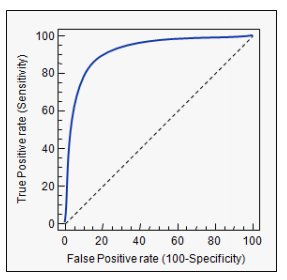
\includegraphics[width=0.55\linewidth]{images/ROCcurve}
\caption{}
\label{fig:roccurve}
\end{figure}
\begin{itemize}
	\item In a Receiver Operating Characteristic (ROC) curve the true positive rate
	(Sensitivity) is plotted in function of the false positive rate (100-Specificity)
	for different cut-off points. 
	\item Each point on the ROC curve represents a sensitivity/specificity
	pair corresponding to a particular decision threshold. 
	\item A
	test with perfect discrimination (no overlap in the two distributions) has a
	ROC curve that passes through the upper left corner (100\% sensitivity, 100\%
	specificity). 
	\item Therefore the closer the ROC curve is to the upper left corner,
	the higher the overall accuracy of the test. %(Zweig and Campbell, 1993).
\end{itemize}

\subsection*{Accuracy, Recall and Precision: An Example}
Calculating precision and recall is actually quite easy. Imagine there are
135 positive cases among 10,000 cases. You want to predict which ones are
positive, and you pick 265 to have a better chance of catching many of the
135 positive cases. You record the IDs of your predictions, and when you
get the actual results you sum up how many times you were right or wrong.
There are four ways of being right or wrong:
\begin{itemize}
\item TN / True Negative: case was negative and predicted negative
\item TP / True Positive: case was positive and predicted positive
\item  FN / False Negative: case was positive but predicted negative
\item FP / False Positive: case was negative but predicted positive
\end{itemize}
Now count how many of the 10,000 cases fall in each category:
\begin{center}
\begin{tabular}{|c|c|c|} \hline
  & Predicted Negative & Predicted Positive \\ \hline
Negative Cases & TN: 9,700 & FP: 165 \\ \hline
Positive Cases &  FN: 35 & TP: 100 \\ \hline
\end{tabular}
\end{center}

\begin{itemize}
	\item What percent of your predictions were correct? \\The accuracy was (9,760+60) out of 10,000 = 98.00\%
	\item	What percent of the positive cases did you catch?\\
 The recall was 100 out of 135 = 74.07\%
	\item	What percent of positive predictions were correct?\\
 The precision was 100 out of 265 = 37.74\%
	\item 	What percent of negative predictions were correct?\\
 The specifity was 9700 out of 9735 = 99.64\%
\end{itemize}
\subsection*{Class Imbalance}
A data set said to be highly skewed if sample from one class is in higher number than other. In an imbalanced data set the class having more number of instances is called as major class while the one having relatively less number of instances are called as minor class .
Applications such as medical diagnosis prediction of rare but important disease is very important than regular treatment. Similar situations are observed in other areas, such as detecting fraud in banking operations, detecting network intrusions, managing risk and predicting failures of technical equipment. 
 In such situation most of the binary classifier are biased towards the major classes and hence show very poor classification rates on minor classes. It is also possible that classifier predicts everything as major class and ignores the minor class completely.
The Accuracy measure is an example of an metric that is affected by this bias. As the F-measure is not computed using the True Negatives, it is less Biased.


\subsection*{The F Score}
The F-score or F-measure is a measure of a classification procedure’s accuracy.
It considers both the precision and the recall to compute the score.
\[ F = \frac{2 \times \mbox{precision} \times \mbox{recall}}{\mbox{precision} + \mbox{recall}}\]

%---------------------------------------------------------- %
\newpage
\section{Model Accuracy}
%http://www.unt.edu/rss/class/Jon/Benchmarks/CrossValidation1_JDS_May2011.pdf
Prediction error refers to the discrepancy or difference between a predicted value (based on a
model) and the actual value. In the standard regression situation, prediction error refers to how
well our regression equation predicts the outcome variable scores of new cases based on
applying the model (coefficients) to the new cases’ predictor variable scores.

\begin{equation}
\text{Accuracy}=\frac{TP+TN}{TP+FP+FN+TN}
\end{equation}

\begin{equation}
\text{Precision}=\frac{TP}{TP+FP} \, 
\end{equation}

\begin{equation}
\text{Recall}=\frac{TP}{TP+FN} \, 
\end{equation}
\section{Recall and Precision}
In a classification task, the precision for a class is the number of true positives (i.e. the number of items correctly labeled as belonging to the positive class) divided by the total number of elements labeled as belonging to the positive class (i.e. the sum of true positives and false positives, which are items incorrectly labeled as belonging to the class). 


\subsection*{Recall}
Recall in this context is defined as the number of true positives divided by the total number of elements that actually belong to the positive class (i.e. the sum of true positives and false negatives, which are items which were not labeled as belonging to the positive class but should have been).

\subsection*{ Cross Validation}
When prediction
is perfect all cases will lie on the diagonal. The percentage of cases on the
diagonal is the percentage of correct classifications. The cross validated set of
data is a more honest presentation of the power of the discriminant function
than that provided by the original classifications and often produces a poorer
outcome. The cross validation is often termed a jack-knife classification, in
that it successively classifies all cases but one to develop a discriminant
function and then categorizes the case that was left out. This process is
repeated with each case left out in turn.This is known as leave-1-out cross
validation.
This cross validation produces a more reliable function. The argument
behind it is that one should not use the case you are trying to predict as part
of the categorization process.
\subsection*{Error Rates}
\begin{itemize}
	\item We can evaluate error rates by means of a training sample (to construct the
	discrimination rule) and a test sample.
	\item An optimistic error rate is obtained by reclassifying the training data. (In
	the training data sets, how many cases were misclassified). This is known
	as the apparent error rate.
	\item The apparent error rate is obtained by using in the training set to estimate
	the error rates. It can be severely optimistically biased, particularly for
	complex classifiers, and in the presence of over-fitted models.
	\item If an independent test sample is used for classifying, we arrive at the true
	error rate.
		\item The true error rate (or conditional error rate) of a classifier is the
	expected probability of misclassifying a randomly selected pattern. It is the
	error rate of an infinitely large test set drawn from the same distribution as
	the training data.
\end{itemize}


\subsection*{Definitions}
\textbf{Accuracy Rate}\\
The accuracy rate calculates the proportion ofobservations being allocated to the \textbf{correct} group by the predictive model. It is calculated as follows:
\[ \frac{
\mbox{Number of Correct Classifications }}{\mbox{Total Number of Classifications }} \]

\[ = \frac{TP + TN}{TP+FP+TN+FN}\]

\newpage

%--------------------------------%

%\frametitle{Sensitivity and Specificity}

 \textbf{Binary Classification Prediction Procedure} Positive or Negative \\ \bigskip
 \textbf{Possible Outcomes from Classification Procedure:}\\ \bigskip
\begin{description}
\item[TN] True Negatives - correct prediction
\item[TP] True Positives - correct prediction
\item[FN] False Negatives - incorrect prediction
\item[FP] False Positives - incorrect prediction
\end{description}




%--------------------------------%


{

\centering
\begin{table}[!htbp]

%\caption{Comparison of percentages.}
\begin{tabular}{c | *2c }
%\toprule
Actual  & \multicolumn{2}{c}{Predicted}\\
Class  & \multicolumn{2}{c}{Class}\\

{}   & Negative & Positive       \\
Negative  &  \textbf{TN} & \textbf{FP}  \\
Positive   &  \textbf{FN} & \textbf{TP}  \\
%\bottomrule
\end{tabular}
\end{table}
}
\begin{description}
\item[TN] \textbf{True Negatives} 
\item[TP] \textbf{True Positives} 
\item[FN] \textbf{False Negatives}
\item[FP] \textbf{False Positives} 
\end{description}



%-------------------------------------------%



\begin{itemize}
\item The F-score or F-measure is a single measure of a classification procedure's usefulness. 
\item The F-score considers both the \textit{\textbf{Precision}} and the \textit{\textbf{Recall}} of the procedure to compute the score.
\item The higher the F-score, the better the predictive power of the 
classification procedure. 
\item A score of 1 means the classification procedure is perfect. The lowest possible F-score is 0.
\[ 0 \leq F \leq 1 \]
\end{itemize}

%-------------------------------------------%



\begin{itemize}
\item \textbf{Precision} is the number of correct positive results divided by the number of \textit{\textbf{predicted positive}} results.
\[ \mbox{Precision}= \frac{TP}{TP+FP}  \]
\item \textbf{Recall} is the number of correct positive results divided by the number of \textit{\textbf{actual positive}} results. 
\[ \mbox{Recall}= \frac{TP}{TP+FN}  \]
\end{itemize}

%-------------------------------------------%


 The F-score is the Harmonic mean of Precision and Recall.
\[ F = \frac{2}{\frac{1}{\mbox{Recall}} + \frac{1}{\mbox{Precision}}} \]
Alternatively
\[ F = 2 \times \left( \frac{\mbox{Precision} \times \mbox{Recall}}{\mbox{Precision} + \mbox{Recall}} \right) \] 

%-------------------------------------------%



%--------------------------------%
\begin{framed}

Number of cases: \textbf{100,000}\\ 
\begin{center}

\begin{table}[!h]
%\caption{Comparison of percentages.}
\begin{tabular}{c *4c}

Actual &  \multicolumn{2}{c}{Predicted} & \multicolumn{2}{c}{Predicted}\\
State &  \multicolumn{2}{c}{Negative} & \multicolumn{2}{c}{Positive}\\

Negative   & \phantom{spa} TN & \textbf{97750}\phantom{spa}   & FP  & \textbf{150}\\
Positive   & \phantom{spa} FN & \textbf{330} \phantom{spa}   & TP  & \textbf{1770}\\

%3   &  6.6  &  5.6   & 35.9  & 37.4\\

\end{tabular}
\end{table}
\end{center}
\end{framed}

\begin{itemize}
\item \textbf{Accuracy} = 0.9952
\item \textbf{Recall} = 0.8428
\item \textbf{Precision} = 0.9218
\end{itemize}

%--------------------------------%



\[ F = 2 \times \frac{\mbox{Precision} \times \mbox{Recall}}{\mbox{Precision} + \mbox{Recall}}\]\bigskip
\[ F = 2 \times \frac{\mbox{0.9218} \times \mbox{0.8428}}{\mbox{0.9218} + \mbox{0.8428}}\] 







\[ F = 2 \times \left( \frac{\mbox{0.9218} \times \mbox{0.8428}}{\mbox{0.9218} + \mbox{0.8428}} \right)\] 

\[ F = 2 \times \left( \frac{0.7770}{1.7646} \right) = 2 \times 0.4402 \]
{
\huge
\[F = 0.8804\] 
}

%--------------------------------%

\noindent \textbf{Misclassification Rate}\\
The misclassification rate calculates the proportion ofobservations being allocated to the \textbf{incorrect} group by the predictive model. It is calculated as follows:
\[ \frac{
\mbox{Number of Incorrect Classifications }}{\mbox{Total Number of Classifications }} \]

\[ = \frac{FP + FN}{TP+FP+TN+FN}\]


\subsection{Roc Curves}
In statistics, a receiver operating characteristic (ROC), or ROC curve, is a graphical plot that illustrates the performance of a binary classifier system as its discrimination threshold is varied. The curve is created by plotting the true positive rate against the false positive rate at various threshold settings. (The true-positive rate is also known as sensitivity in biomedicine, or recall in machine learning. The false-positive rate is also known as the fall-out and can be calculated as 1 - specificity). 

The ROC curve is thus the sensitivity as a function of fall-out. In general, if the probability distributions for both detection and false alarm are known, the ROC curve can be generated by plotting the cumulative distribution function (area under the probability distribution from $-\infty$ to +$$\infty$) of the detection probability in the y-axis versus the cumulative distribution function of the false-alarm probability in x-axis.


ROC analysis provides tools to select possibly optimal models and to discard suboptimal ones independently from (and prior to specifying) the cost context or the class distribution. ROC analysis is related in a direct and natural way to cost/benefit analysis of diagnostic decision making.


The ROC curve was first developed by electrical engineers and radar engineers during World War II for detecting enemy objects in battlefields and was soon introduced to psychology to account for perceptual detection of stimuli. ROC analysis since then has been used in medicine, radiology, biometrics, and other areas for many decades and is increasingly used in machine learning and data mining research.
The ROC is also known as a relative operating characteristic curve, because it is a comparison of two operating characteristics (TPR and FPR) as the criterion changes.[1]


\subsection*{Misclassification Cost}
As in all statistical procedures it is helpful to use diagnostic procedures to
asses the efficacy of the discriminant analysis. We use cross-validation to
assess the classification probability. Typically you are going to have some
prior rule as to what is an acceptable misclassification rate.
Those rules might involve things like, “what is the cost of misclassification?”
Consider a medical study where you might be able to diagnose cancer.
There are really two alternative costs. The cost of misclassifying someone
as having cancer when they don’t. This could cause a certain amount of emotional
grief. Additionally there would be the substantial cost of unnecessary
treatment.
\smallskip 
There is also the alternative cost of misclassifying someone as not having
cancer when in fact they do have it.
A good classification procedure should
\begin{itemize}
	\item result in few misclassifications
	\item take prior probabilities of occurrence into account
	\item consider the cost of misclassification
\end{itemize}
For example, suppose there tend to be more financially sound firms than
bankrupt firm. If we really believe that the prior probability of a financially
distressed and ultimately bankrupted firm is very small, then one should classify
a randomly selected firm as non-bankrupt unless the data overwhelmingly
favor bankruptcy.
\smallskip 
There are two costs associated with discriminant analysis classification:
The \textbf{true misclassification cost per class}, and the\textbf{ expected misclassification
cost} (ECM) per observation.

\smallskip

Suppose there we have a binary classification system, with two classes:
class 1 and class 2. Suppose that classifying a class 1 object as belonging
to class 2 represents a more serious error than classifying a class 2 object as
belonging to class 1. There would an assignable cost to each error. c(i|j) is
the cost of classifying an observation into class j if its true class is i. The
costs of misclassification can be defined by a cost matrix.
\begin{center}

\begin{tabular}{|c|c|c|}	\hline 
	& Predicted & Predicted \\ 
	& Class 1 & Class 2 \\ \hline 
	Class 1 & 0&  c(2|1) \\ \hline 
	Class 2 & c(1|2) & 0 \\ \hline 
\end{tabular}
\end{center}


\subsection*{ Expected Cost of Misclassification (ECM)}
Let p1 and p2 be the prior probability of class 1 and class 2 respectively.
Necessarily p1 + p2 = 1.

The conditional probability of classifying an object as class 1 when it is
in fact from class 2 is denoted p(1|2). Similarly the conditional probability
of classifying an object as class 2 when it is in fact from class 1 is denoted
p(2|1).
\[ ECM = c(2|1)p(2|1)p1 + c(1|2)p(1|2)p2\]
(In other words: the sum of the cost of misclassification times the (joint)
probability of that misclassification.
A reasonable classification rule should have ECM as small as possible.
\end{document}